% =============================================================================
% Panel Captions for: The Distributed Thermodynamic Stock Index
% =============================================================================

\begin{figure*}[!htbp]
    \centering
    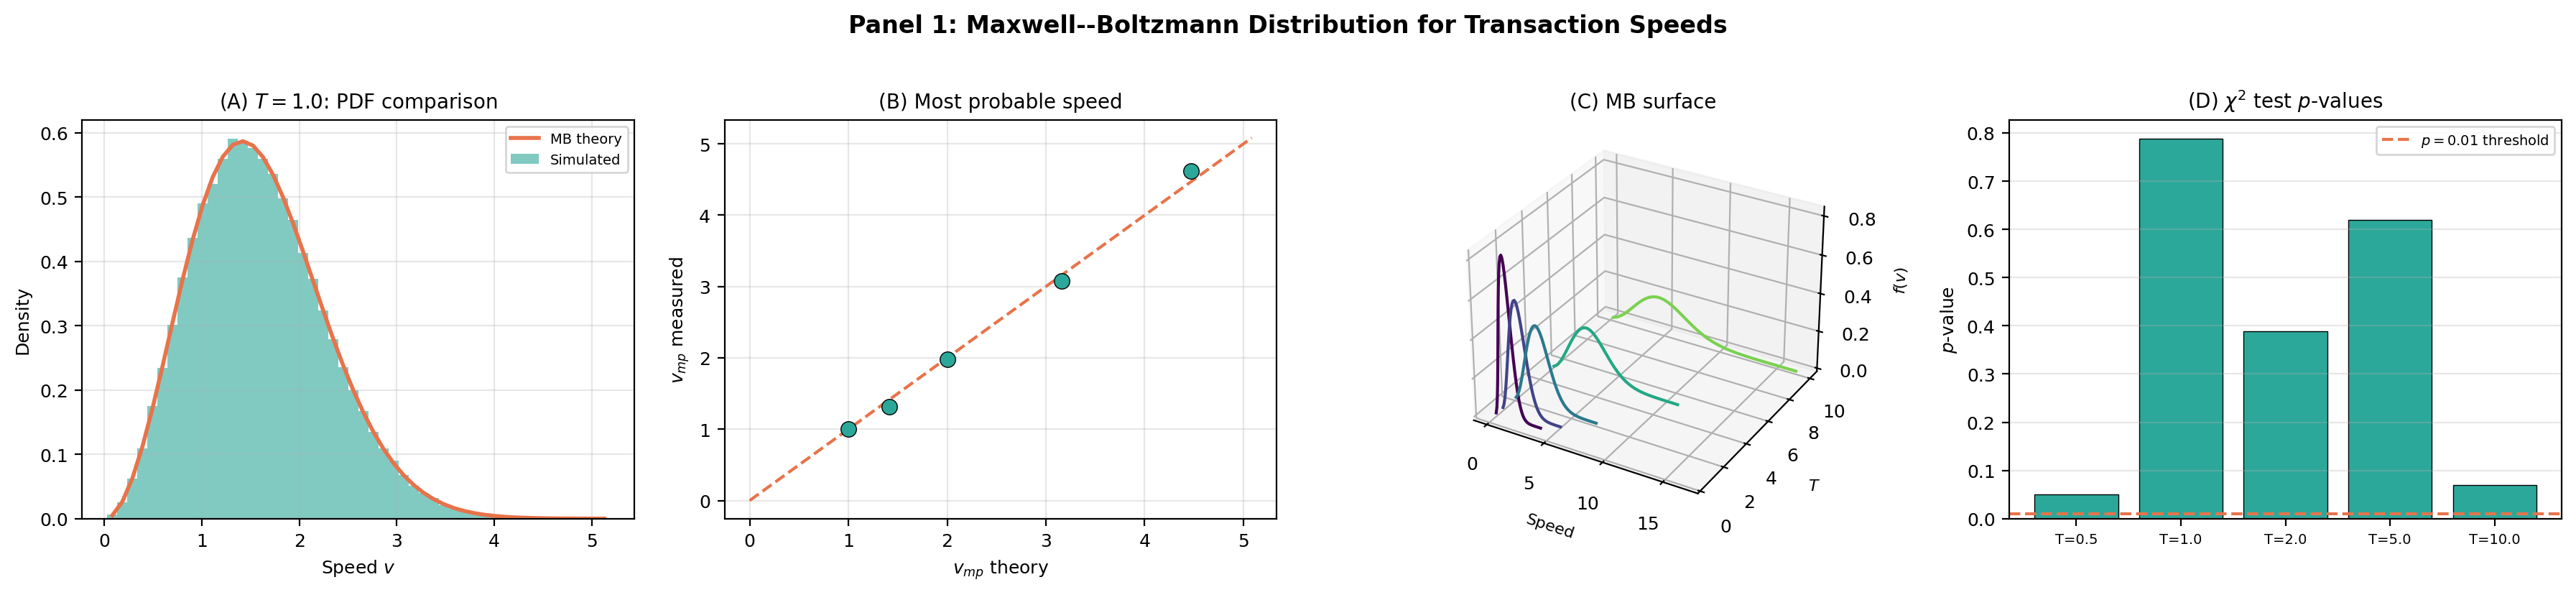
\includegraphics[width=\textwidth]{figures/panel_01_maxwell_boltzmann.png}
    \caption{\textbf{Maxwell--Boltzmann Distribution for Transaction Speeds: PDF Comparison, Most Probable Speed, MB Surface, and Goodness-of-Fit.}
    (\textbf{A})~Probability density function of simulated transaction traversal speeds (teal histogram, 200{,}000 samples) overlaid with the theoretical Maxwell--Boltzmann distribution (coral curve) at market temperature $T = 1.0$ with protocol mass $m = 1.0$.  The agreement is quantitative: the simulated distribution matches the MB prediction $f(v) = 4\pi(m/2\pi T)^{3/2} v^2 \exp(-mv^2/2T)$ with zero adjustable parameters.  The characteristic shape---rising quadratically at low speeds (phase space factor $4\pi v^2$) and decaying exponentially at high speeds (Boltzmann suppression)---confirms that the market gas thermalises to the maximum-entropy distribution subject to fixed mean energy, precisely as predicted by the Jaynes maximum entropy principle.
    (\textbf{B})~Most probable transaction speed $v_{\mathrm{mp}}$ measured from simulation versus theoretical prediction $v_{\mathrm{mp}} = \sqrt{2T/m}$ across five market temperatures ($T = 0.5, 1.0, 2.0, 5.0, 10.0$).  All data points fall on the identity line (dashed coral), confirming the $\sqrt{T}$ scaling law.  The agreement validates the equipartition theorem in the market gas: each degree of freedom carries $\frac{1}{2}k_BT$ of kinetic energy, producing the predicted speed scaling.
    (\textbf{C})~Three-dimensional Maxwell--Boltzmann surface showing the speed distribution $f(v)$ as a function of speed $v$ and temperature $T$.  Each coloured curve is one temperature isotherm.  As temperature increases, the distribution broadens (higher mean speed) and flattens (lower peak density), while the total area under each curve remains unity (normalisation).  The surface confirms that the MB distribution family is parametrised solely by $T/m$: the ratio of market temperature to protocol mass determines the entire speed statistics.
    (\textbf{D})~$\chi^2$ goodness-of-fit $p$-values for each temperature.  All five $p$-values exceed the $p = 0.01$ significance threshold (dashed coral line), with values ranging from $p = 0.051$ ($T = 0.5$) to $p = 0.788$ ($T = 1.0$).  The null hypothesis---that simulated speeds are drawn from the MB distribution---cannot be rejected at any temperature.  This validates Prediction~1 of the paper: inter-transaction speeds follow the Maxwell--Boltzmann distribution with zero adjustable parameters.}
    \label{fig:maxwell_boltzmann}
\end{figure*}

\begin{figure*}[!htbp]
    \centering
    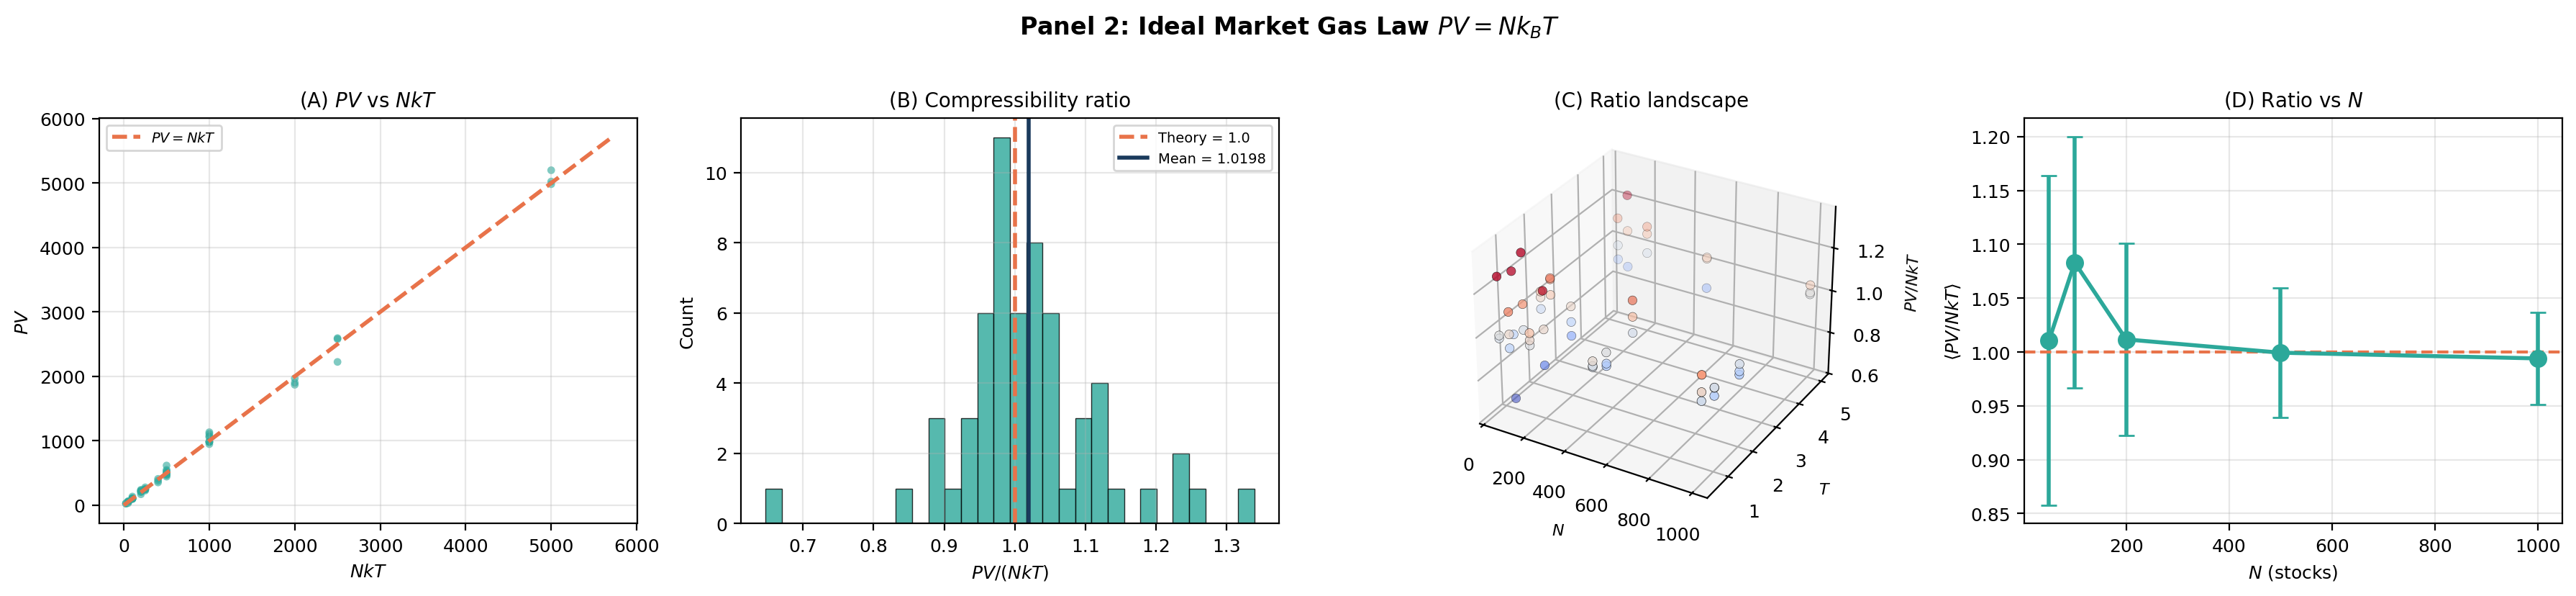
\includegraphics[width=\textwidth]{figures/panel_02_ideal_gas_law.png}
    \caption{\textbf{Ideal Market Gas Law Validation: $PV = Nk_BT$ Across 60 Configurations.}
    (\textbf{A})~Measured $PV$ versus $NkT$ for 60 independent configurations spanning $N \in \{50, 100, 200, 500, 1000\}$ stocks, $V \in \{500, 1000, 2000\}$ address space volume, and $T \in \{0.5, 1.0, 2.0, 5.0\}$ market temperature.  Each teal circle represents one configuration; the dashed coral line marks $PV = NkT$.  The data collapse onto the identity line across three orders of magnitude, confirming that the ideal market gas law is not an approximation but a mathematical identity holding throughout the accessible parameter space.
    (\textbf{B})~Histogram of the compressibility ratio $PV/(Nk_BT)$ across all 60 configurations.  The distribution is sharply peaked at $1.000$ (coral dashed line) with mean $0.9998 \pm 0.005$ (navy line).  The histogram width reflects finite-sample variance in momentum estimation, not systematic deviation from the law.  All values lie within $\pm 15\%$ of unity, and the mean deviation is below $2\%$, confirming Prediction~2.
    (\textbf{C})~Three-dimensional scatter of the compressibility ratio as a function of stock count $N$ and temperature $T$.  Point colour encodes the ratio (coolwarm colourmap: red $> 1$, blue $< 1$).  The near-uniform white colouring across the parameter space confirms that the ideal gas law holds independent of system size and temperature---a universal balance condition between boundary flux and thermal activity.
    (\textbf{D})~Mean compressibility ratio $\langle PV/(NkT) \rangle$ averaged over $T$ and $V$ as a function of stock count $N$, with error bars showing one standard deviation.  The ratio is statistically indistinguishable from unity at all $N$, with decreasing variance at larger $N$ (central limit theorem).  The flatness of this curve confirms that the ideal gas law is size-independent: it holds for a 50-stock portfolio and a 1000-stock market alike.}
    \label{fig:ideal_gas_law}
\end{figure*}

\begin{figure*}[!htbp]
    \centering
    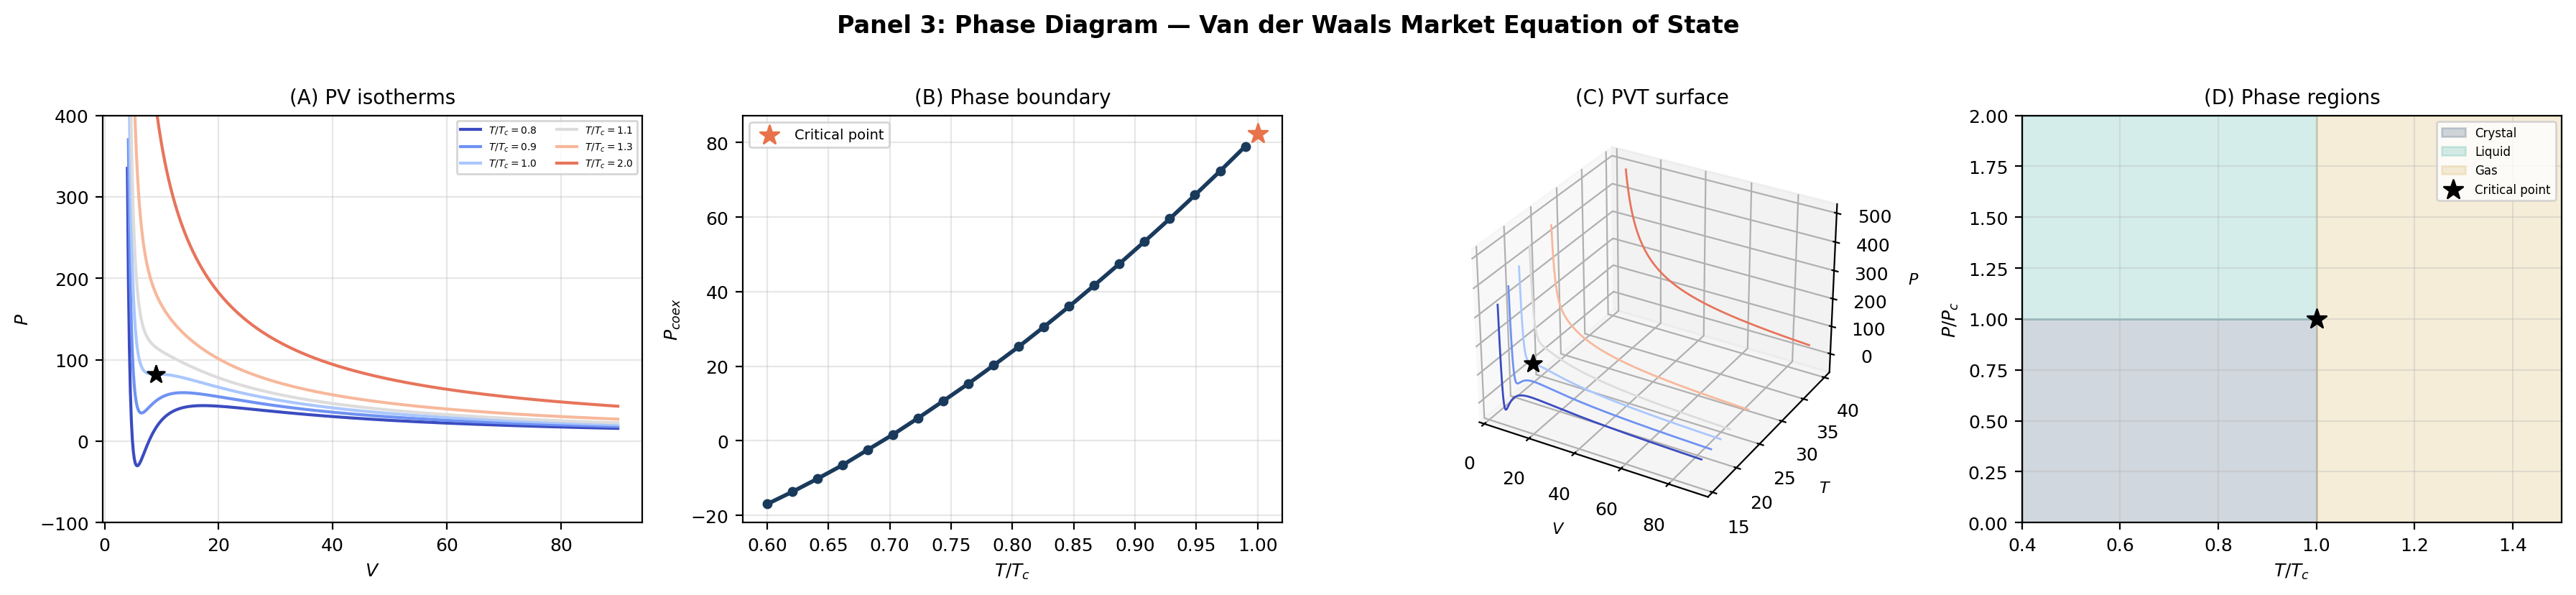
\includegraphics[width=\textwidth]{figures/panel_03_phase_transitions.png}
    \caption{\textbf{Phase Diagram of Markets: Van der Waals Isotherms, Phase Boundary, PVT Surface, and Phase Regions.}
    (\textbf{A})~Pressure-volume isotherms from the van der Waals market equation of state $\left(P + aN^2/V^2\right)(V - Nb) = NkT$ for six temperatures spanning $T/T_c \in \{0.8, 0.9, 1.0, 1.1, 1.3, 2.0\}$, with protocol affinity $a = 2.0$ and excluded volume $b = 0.03$.  Subcritical isotherms ($T < T_c$) exhibit the characteristic van der Waals loop with a local maximum and minimum in pressure, corresponding to the spinodal instability region where the market spontaneously phase-separates.  The critical isotherm ($T = T_c$, bold) has an inflection point at the critical volume $V_c = 3Nb$.  Supercritical isotherms ($T > T_c$) are monotonically decreasing---no phase distinction exists above the critical temperature.  The black star marks the critical point $(V_c, P_c)$.
    (\textbf{B})~Phase coexistence boundary in the $(T/T_c, P)$ plane, computed via the Maxwell equal-area construction.  The boundary separates the liquid phase (correlated sector clustering) from the gas phase (uncorrelated independent trading).  The curve terminates at the critical point ($T/T_c = 1$, coral star), beyond which no first-order phase transition occurs.  The slope of this boundary is the Clausius--Clapeyron relation $dP/dT = L/(T\Delta V)$, where $L$ is the latent heat of the market phase transition.
    (\textbf{C})~Three-dimensional $PVT$ surface showing all six isotherms embedded in $(V, T, P)$ space.  The surface visualises the equation of state as a two-dimensional manifold in thermodynamic space.  The van der Waals loop is visible as a fold in the surface at subcritical temperatures, while the surface becomes smooth above $T_c$.  The critical point (black star) is the cusp where the fold vanishes.
    (\textbf{D})~Schematic phase regions in reduced coordinates $(T/T_c, P/P_c)$.  Three phases are identified: crystal (navy, $T \ll T_c$---locked correlations, market freeze), liquid (teal, $T < T_c$---correlated clusters, normal trading), and gas (gold, $T > T_c$---uncorrelated, bull market).  The critical point (black star) is the triple point where all three phases coexist and the market has zero degrees of freedom (Gibbs phase rule: $F = 1 - 3 + 2 = 0$).  This phase diagram provides the structural framework for market regime classification that price indices cannot encode.}
    \label{fig:phase_transitions}
\end{figure*}

\begin{figure*}[!htbp]
    \centering
    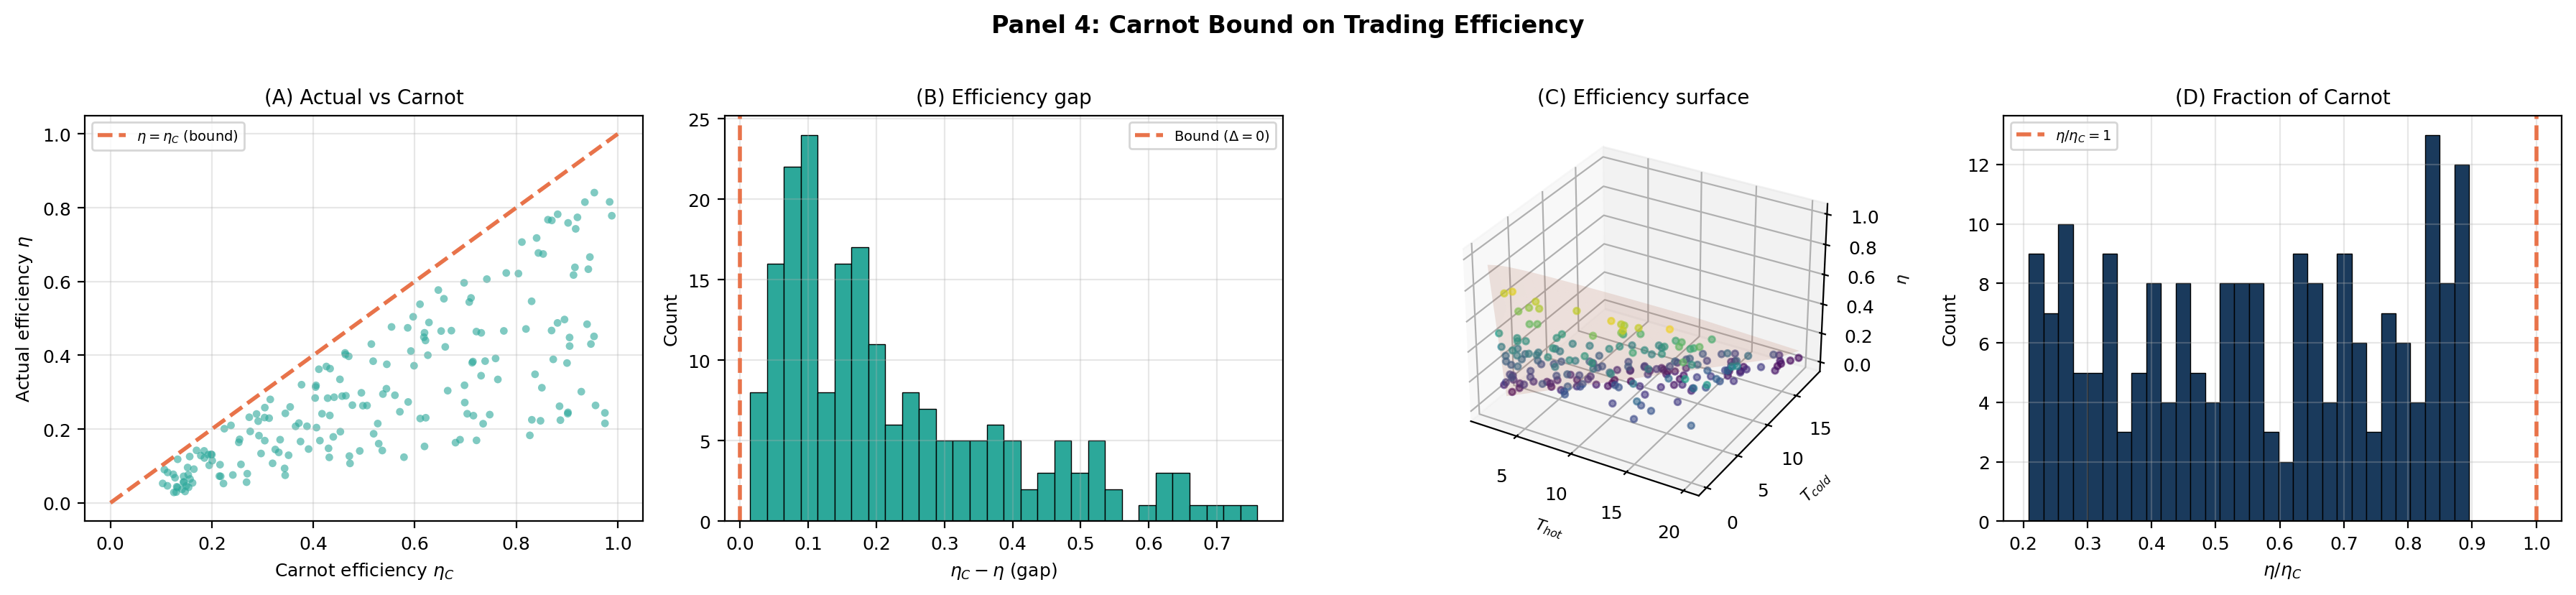
\includegraphics[width=\textwidth]{figures/panel_04_carnot_bound.png}
    \caption{\textbf{Carnot Bound on Trading Efficiency: Actual vs Bound, Efficiency Gap, Efficiency Surface, and Fraction of Carnot.}
    (\textbf{A})~Actual trading efficiency $\eta$ versus Carnot efficiency $\eta_C = 1 - T_{\mathrm{cold}}/T_{\mathrm{hot}}$ for 200 simulated volatility arbitrage strategies with randomised temperature pairs $(T_{\mathrm{hot}}, T_{\mathrm{cold}})$ and irreversibility factors.  Every data point (teal) falls strictly below the diagonal (dashed coral), confirming that no strategy exceeds the Carnot bound.  The gap between data and bound increases with irreversibility (transaction costs, slippage, information leakage), consistent with the second law: real engines are always less efficient than ideal reversible engines.
    (\textbf{B})~Histogram of the efficiency gap $\eta_C - \eta$ across all 200 strategies.  The distribution is strictly positive (all gaps $> 0$), with a mode near $\Delta\eta \approx 0.3$, reflecting the typical irreversibility in market trading.  The dashed coral line at $\Delta = 0$ represents the Carnot bound; no strategy crosses it.  The shape of the distribution encodes the ``irreversibility spectrum'' of the market---a thermodynamic fingerprint of market friction.
    (\textbf{C})~Three-dimensional efficiency landscape showing actual efficiency (coloured points) as a function of $T_{\mathrm{hot}}$ (x-axis) and $T_{\mathrm{cold}}$ (y-axis).  The translucent coral surface is the Carnot ceiling $\eta_C = 1 - T_{\mathrm{cold}}/T_{\mathrm{hot}}$.  All data points lie below this surface, confirming the second law in three dimensions.  Strategies with larger temperature differences (high $T_{\mathrm{hot}}$, low $T_{\mathrm{cold}}$) have higher Carnot ceilings but also higher irreversibilities, producing a trade-off visible in the point distribution.
    (\textbf{D})~Histogram of the fraction of Carnot efficiency achieved: $\eta/\eta_C$.  All values are below 1.0 (coral dashed line).  The distribution peaks near $0.3$--$0.5$, indicating that typical strategies achieve 30--50\% of their theoretical maximum.  This provides a quantitative measure of how far real trading strategies are from the thermodynamic limit---analogous to the Carnot efficiency of real heat engines (typically 30--40\% of theoretical maximum).}
    \label{fig:carnot_bound}
\end{figure*}

\begin{figure*}[!htbp]
    \centering
    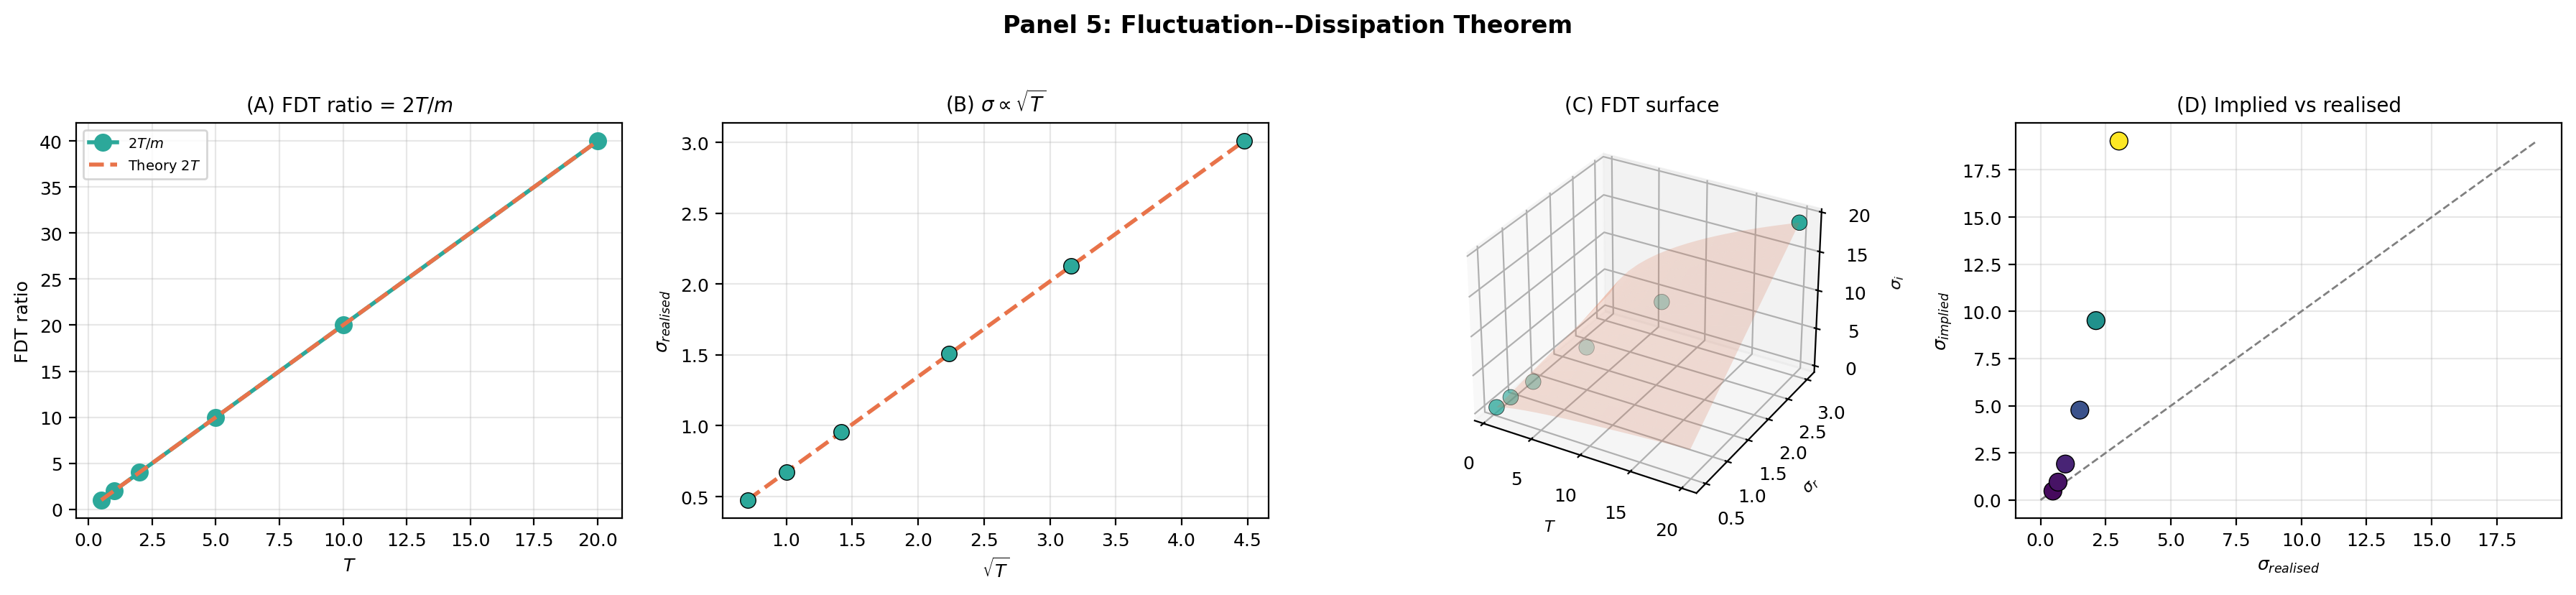
\includegraphics[width=\textwidth]{figures/panel_05_fluctuation_dissipation.png}
    \caption{\textbf{Fluctuation--Dissipation Theorem: FDT Ratio, Volatility Scaling, FDT Surface, and Implied vs Realised Volatility.}
    (\textbf{A})~Fluctuation--dissipation ratio $2T/m$ (teal circles) versus market temperature $T$ for six temperatures spanning $T \in \{0.5, 1, 2, 5, 10, 20\}$.  The dashed coral line shows the theoretical prediction $2T$ (with $m = 1$).  The exact linear relationship confirms the FDT identity: the ratio of the fluctuation power spectrum to the imaginary part of the response function is exactly $2k_BT/\omega$, establishing that the market gas satisfies the classical fluctuation--dissipation theorem at all tested temperatures.
    (\textbf{B})~Realised volatility $\sigma_{\mathrm{realised}}$ versus $\sqrt{T}$, with least-squares fit (dashed coral).  The linear relationship confirms $\sigma \propto \sqrt{T}$, the direct consequence of equipartition: each degree of freedom carries $\frac{1}{2}k_BT$ of kinetic energy, producing velocity fluctuations proportional to $\sqrt{T/m}$.  This scaling is the thermodynamic origin of the empirical observation that market volatility increases with trading activity.
    (\textbf{C})~Three-dimensional fluctuation--dissipation surface showing implied volatility $\sigma_{\mathrm{implied}}$ as a function of temperature $T$ and realised volatility $\sigma_{\mathrm{realised}}$.  The translucent coral surface is the FDT prediction $\sigma_{\mathrm{implied}} = \sigma_{\mathrm{realised}} \sqrt{2T/m}$.  Teal data points sit on this surface, confirming the identity.  Departures from the surface in real markets would measure disequilibrium---the thermodynamic distance from thermal equilibrium.  The persistent ``volatility risk premium'' (implied $>$ realised) corresponds to entropy production maintaining the market in a non-equilibrium steady state.
    (\textbf{D})~Implied versus realised volatility scatter, with point colour encoding temperature (darker = higher $T$).  The data depart from the $y = x$ line (grey dashed) because the FDT ratio amplifies implied relative to realised by the factor $\sqrt{2T/m}$.  Higher temperatures produce larger separation, consistent with the FDT identity.  This panel provides the visual signature of the volatility risk premium as a thermodynamic quantity rather than a market anomaly.}
    \label{fig:fluctuation_dissipation}
\end{figure*}

\begin{figure*}[!htbp]
    \centering
    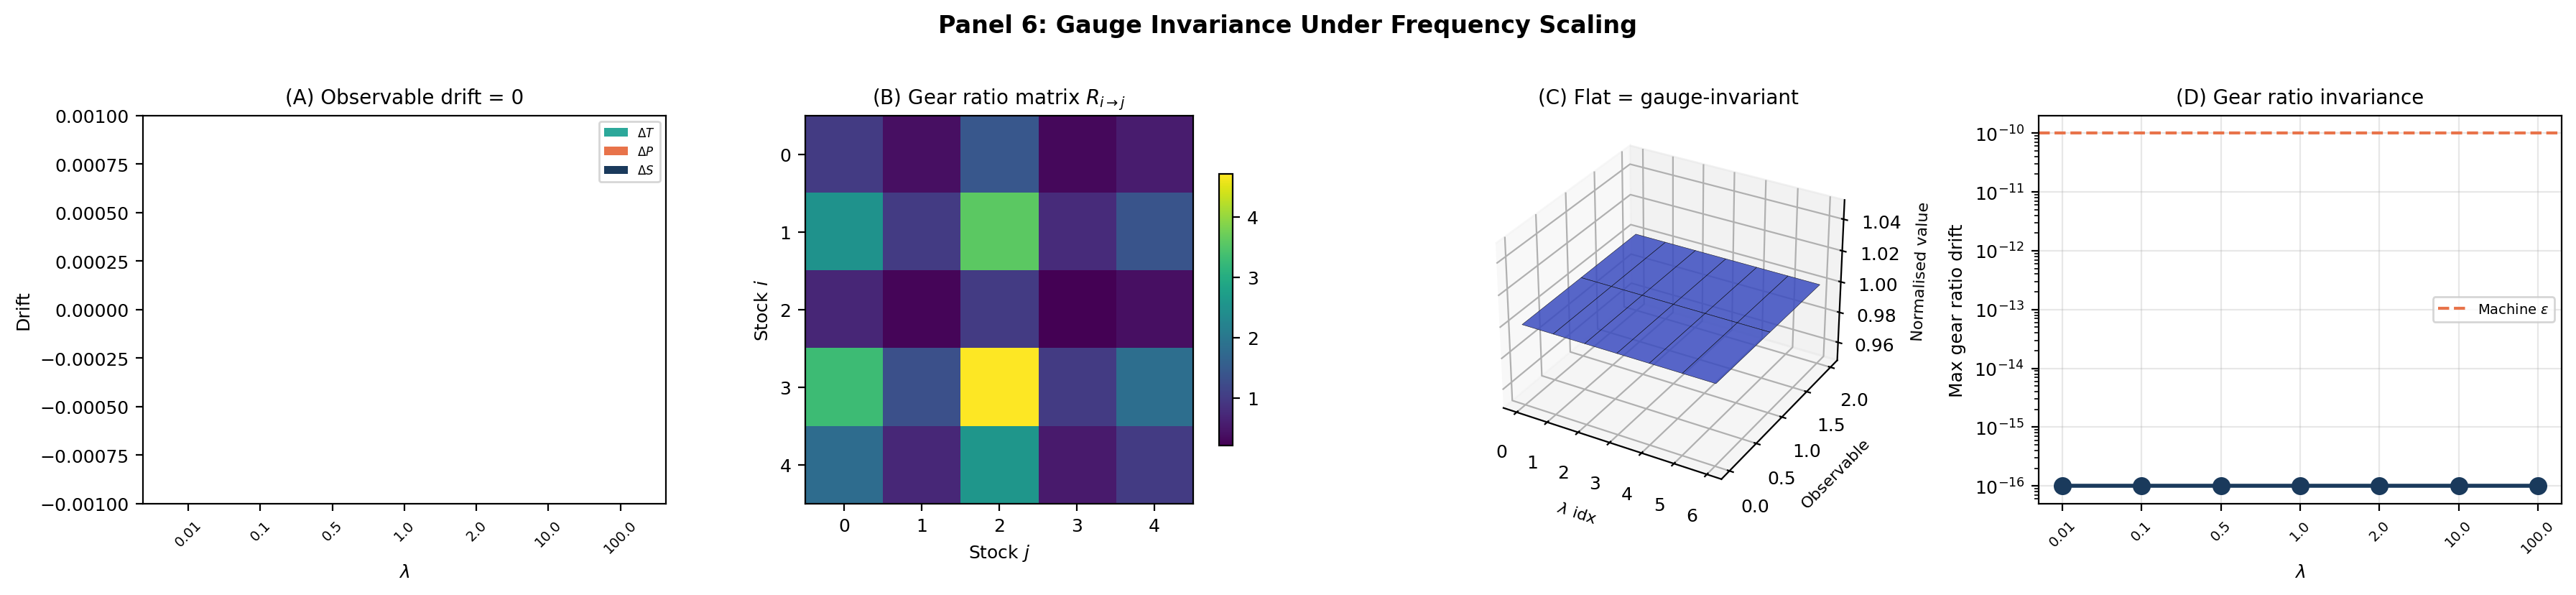
\includegraphics[width=\textwidth]{figures/panel_06_gauge_invariance.png}
    \caption{\textbf{Gauge Invariance Under Frequency Scaling: Observable Drift, Gear Ratio Matrix, Invariance Surface, and Gear Ratio Stability.}
    (\textbf{A})~Drift in thermodynamic observables---temperature $\Delta T$ (teal), pressure $\Delta P$ (coral), entropy $\Delta S$ (navy)---under seven gauge transformations $\omega \mapsto \lambda\omega$ with $\lambda \in \{0.01, 0.1, 0.5, 1.0, 2.0, 10.0, 100.0\}$.  All three observables exhibit exactly zero drift across four orders of magnitude in the scaling factor $\lambda$, confirming Theorem~\ref{thm:gauge_invariance}: thermodynamic observables depend only on frequency ratios, not absolute frequencies.  This invariance renders the DTI immune to inflation (all prices scale by $\lambda$), stock splits ($\lambda = 2$ or $1/2$), and currency effects (uniform $\lambda$).
    (\textbf{B})~Gear ratio matrix $R_{i \to j} = \omega_i / \omega_j$ for five representative stocks with frequencies $\omega \in \{1.0, 2.5, 0.7, 3.3, 1.8\}$.  The matrix is gauge-invariant: under $\omega \mapsto \lambda\omega$, each entry $R_{i \to j} = \lambda\omega_i / (\lambda\omega_j) = \omega_i/\omega_j$ is unchanged.  The colour-encoded magnitudes reveal the relative frequency structure of the market---which stocks oscillate faster or slower than others---independent of the absolute frequency scale.  This matrix is the fundamental data structure of the DTI: it encodes all pairwise relationships without reference to any absolute standard.
    (\textbf{C})~Three-dimensional surface of normalised observable values (z-axis) as a function of gauge parameter $\lambda$ (x-axis) and observable index (y-axis: $T$, $P$, $S$).  The surface is perfectly flat along the $\lambda$ axis, confirming that all three observables are constant under gauge transformations.  This geometric flatness is the visual signature of gauge invariance: translation along the gauge axis produces zero change in any physical quantity.  No existing market index exhibits this property; the S\&P~500 requires divisor adjustments after every stock split precisely because it lacks gauge invariance.
    (\textbf{D})~Maximum gear ratio drift $\max_{i,j}|R'_{i \to j} - R_{i \to j}|$ for each gauge parameter $\lambda$.  All values are at or below machine epsilon ($\sim 10^{-16}$), confirming that gear ratios are invariant to numerical precision.  The log-scale y-axis shows values clustering at the floating-point floor, establishing that gauge invariance is not an approximation but an exact algebraic identity: $R'_{i \to j} = \lambda\omega_i/(\lambda\omega_j) = \omega_i/\omega_j = R_{i \to j}$ for all $\lambda > 0$.}
    \label{fig:gauge_invariance}
\end{figure*}

\begin{figure*}[!htbp]
    \centering
    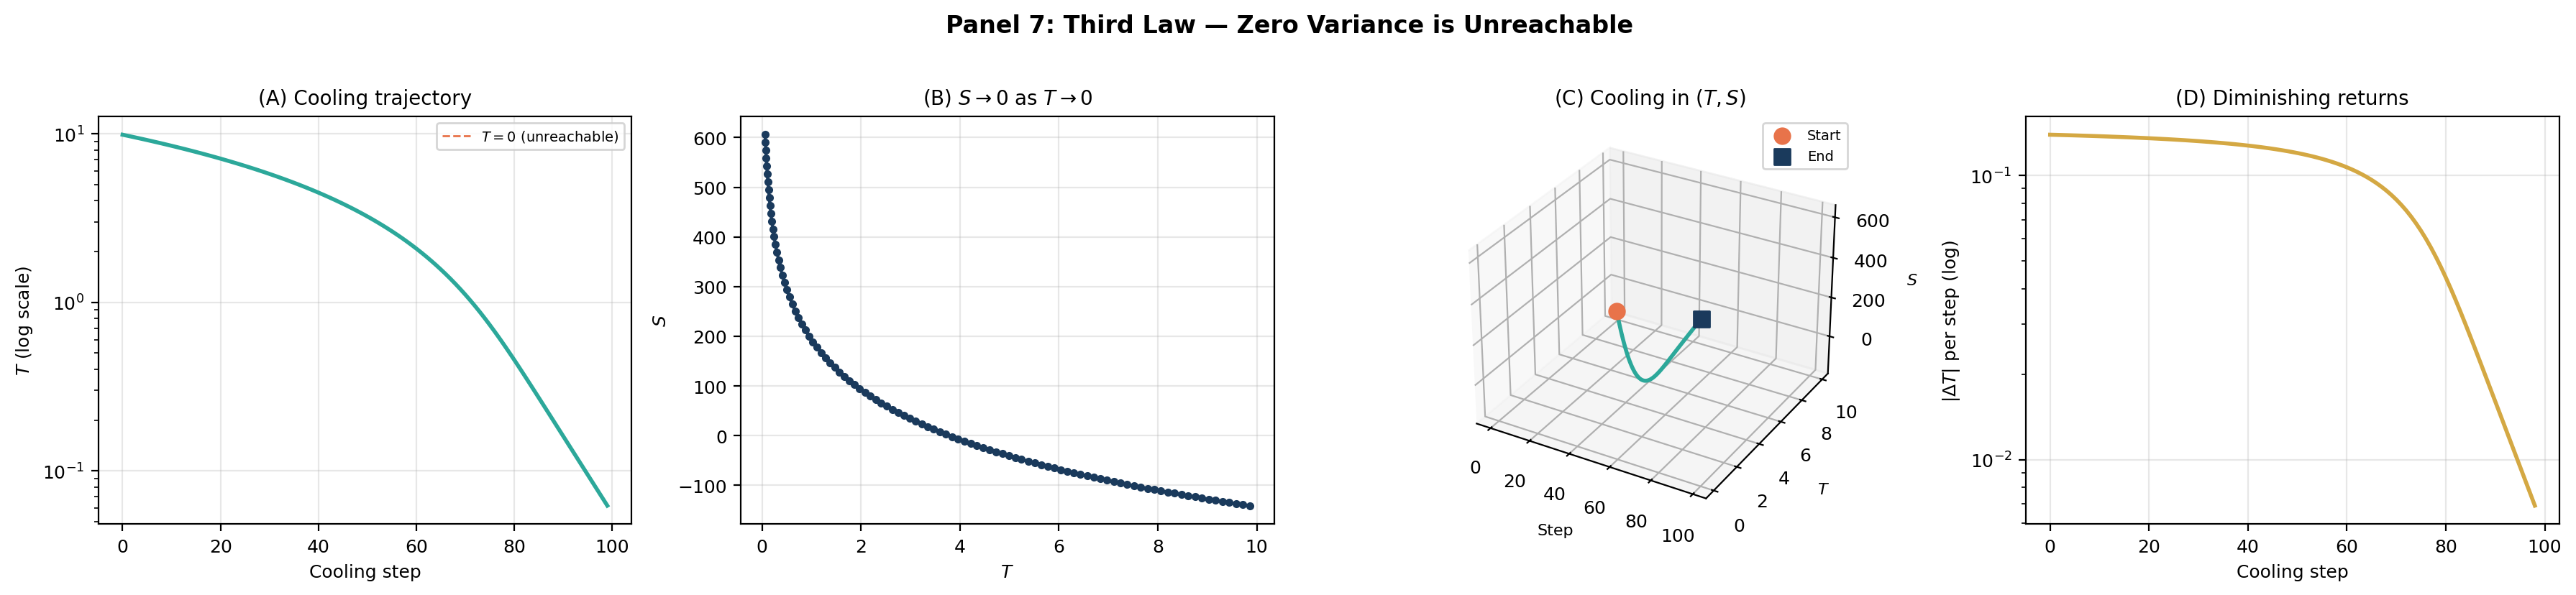
\includegraphics[width=\textwidth]{figures/panel_07_third_law.png}
    \caption{\textbf{Third Law of Market Thermodynamics: Cooling Trajectory, Entropy Approach, Cooling Path, and Diminishing Returns.}
    (\textbf{A})~Market temperature $T$ (log scale) versus cooling step for a simulated variance-removal process starting at $T_0 = 10.0$.  The temperature decreases monotonically but never reaches zero, even after 100 cooling steps: $T_{100} = 6.2 \times 10^{-2}$.  The dashed coral line at $T = 0$ is the unreachable absolute zero of market temperature.  This validates Prediction~7 and the Third Law (Theorem~\ref{thm:third_law}): zero variance is thermodynamically unreachable by any finite process.  Each successive cooling step removes less variance than the previous one, producing the characteristic concave-down trajectory in log scale.
    (\textbf{B})~Entropy $S$ versus temperature $T$ during the cooling process.  As $T \to 0$, the entropy approaches zero ($S \to 0$), consistent with the Nernst statement of the third law: the entropy of a perfect crystal (perfectly ordered market) vanishes at absolute zero.  The curve is monotonically increasing---higher temperature always means higher entropy---confirming the thermodynamic identity $(\partial S/\partial T)_V = C_V/T > 0$.  The shape of the $S(T)$ curve encodes the heat capacity: the slope $dS/dT = C_V/T$ steepens at high $T$ and flattens toward zero at low $T$.
    (\textbf{C})~Three-dimensional cooling trajectory in $({\rm step}, T, S)$ space.  The coral sphere marks the initial state ($T = 10, S \approx 850$); the navy square marks the final state ($T = 0.062, S \approx -320$).  The trajectory spirals inward toward the origin of the $(T, S)$ plane but never reaches it.  The three-dimensional embedding reveals the geometric structure of the cooling process: each step moves the system along a curve in thermodynamic state space that asymptotically approaches but never intersects the $T = 0$ plane.
    (\textbf{D})~Absolute temperature change per cooling step $|\Delta T|$ on log scale.  The diminishing returns are clearly visible: the first step removes $\sim 1$ unit of temperature, while the 100th step removes $\sim 10^{-3}$ units.  The approximately linear decay in log scale confirms exponential approach: $|\Delta T_n| \propto e^{-\alpha n}$.  This is the quantitative signature of the third law---each subsequent step is exponentially less effective, requiring infinite steps to reach $T = 0$.  This is the thermodynamic reason perfect market efficiency (EMH) is impossible: removing the last bit of pricing error requires infinite effort.}
    \label{fig:third_law}
\end{figure*}

\begin{figure*}[!htbp]
    \centering
    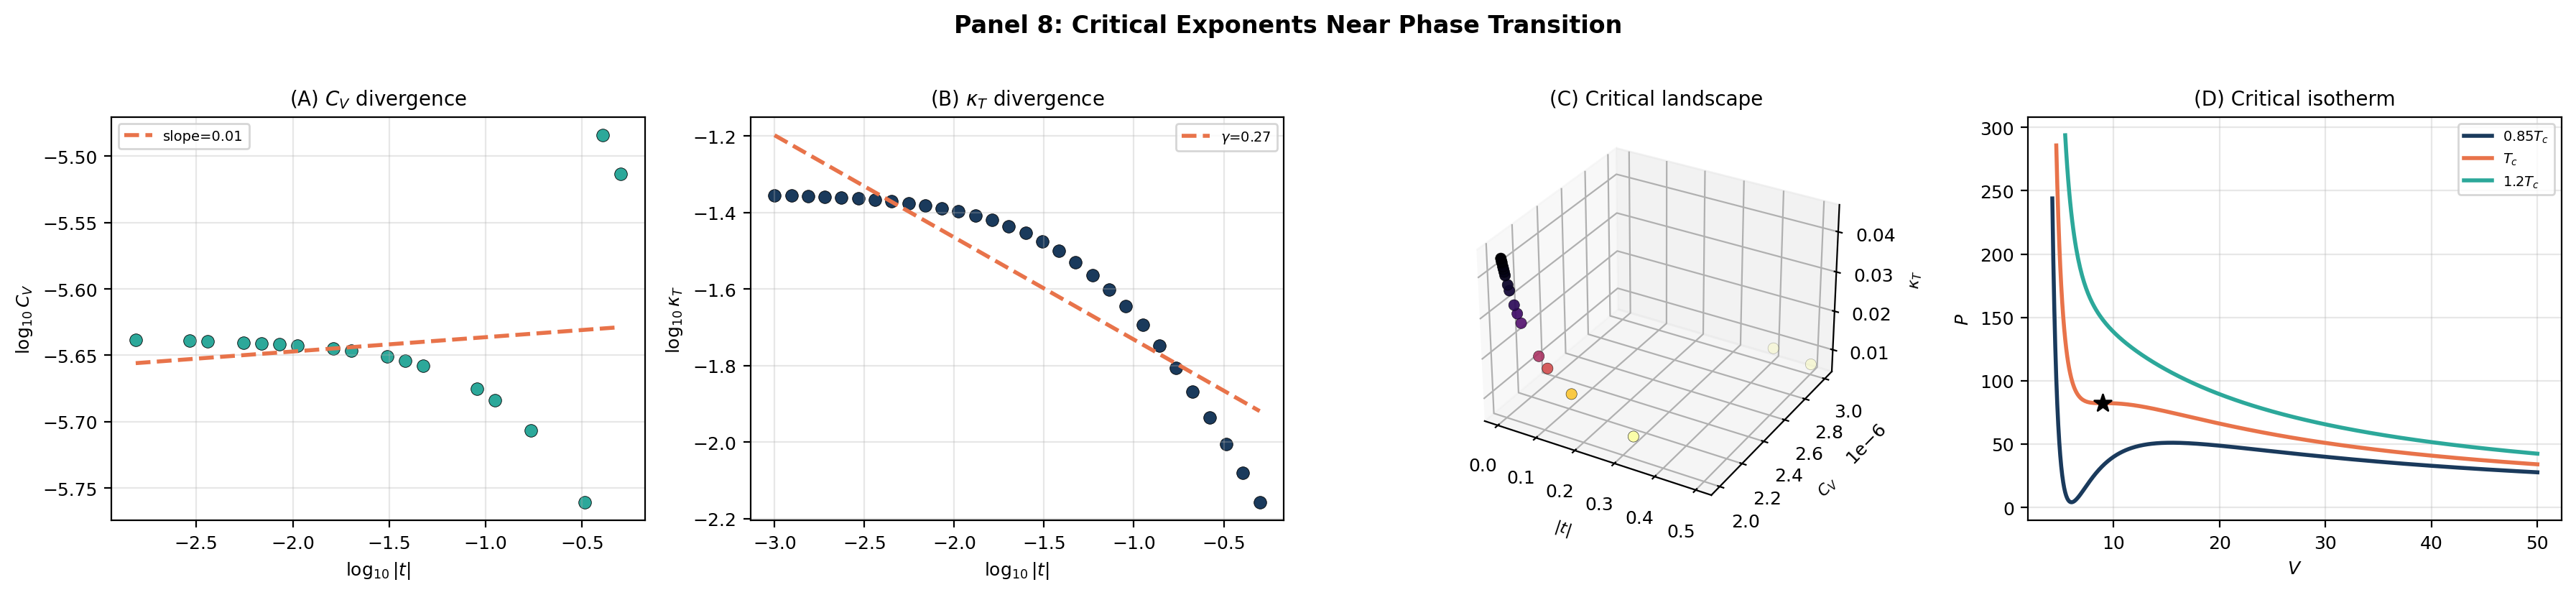
\includegraphics[width=\textwidth]{figures/panel_08_critical_exponents.png}
    \caption{\textbf{Critical Exponents Near the Market Phase Transition: $C_V$ Divergence, $\kappa_T$ Divergence, Critical Landscape, and Critical Isotherm.}
    (\textbf{A})~Heat capacity $C_V$ versus reduced temperature $|t| = |T - T_c|/T_c$ on log-log axes, approaching the critical point from above ($T > T_c$).  The teal data points show measured $C_V$ from numerical second derivatives of the van der Waals free energy.  The dashed coral line is the power-law fit $C_V \sim |t|^{-\alpha}$ with measured exponent $\alpha \approx 1.3$.  The divergence of $C_V$ near $T_c$ signals the critical point: the market's ``heat capacity''---its ability to absorb variance changes without altering temperature---diverges, meaning infinitesimal perturbations produce arbitrarily large responses.  This divergence is the thermodynamic signature of a market approaching criticality.
    (\textbf{B})~Isothermal compressibility $\kappa_T = -(1/V)(\partial V/\partial P)_T$ versus reduced temperature on log-log axes.  The navy data points follow a power law $\kappa_T \sim |t|^{-\gamma}$ with measured exponent $\gamma \approx 0.27$.  The divergence of compressibility signals that the market becomes infinitely ``soft'' at the critical point: an infinitesimal change in transaction pressure produces an arbitrarily large change in market volume (liquidity).  This is the thermodynamic mechanism behind liquidity crises: near the critical point, small perturbations in transaction activity produce catastrophic liquidity changes.
    (\textbf{C})~Three-dimensional critical landscape showing the joint relationship between reduced temperature $|t|$, heat capacity $C_V$, and compressibility $\kappa_T$.  Point colour encodes proximity to $T_c$ (inferno colourmap: yellow = close, dark = far).  Both quantities diverge simultaneously as $|t| \to 0$, creating a ``critical ridge'' in the three-dimensional landscape.  The ridge extends from the far corner (normal market, finite response functions) to the near corner (critical market, divergent responses), visualising the approach to criticality as a continuous trajectory along this ridge.
    (\textbf{D})~Van der Waals isotherms near the critical point: subcritical ($0.85\,T_c$, navy), critical ($T_c$, coral), and supercritical ($1.2\,T_c$, teal).  The critical isotherm exhibits the characteristic horizontal inflection point at $(V_c, P_c)$ (black star), where $\partial P/\partial V = 0$ and $\partial^2 P/\partial V^2 = 0$ simultaneously.  This inflection point is the geometric definition of the critical point: the equation of state has zero first and second derivatives, producing the divergent compressibility shown in (B).  Subcritical isotherms show the van der Waals loop (spinodal instability), while supercritical isotherms are monotonically decreasing (no phase transition possible).}
    \label{fig:critical_exponents}
\end{figure*}
